\documentclass{beamer}
\usepackage{amsmath}
\usepackage[english]{babel} %set language; note: after changing this, you need to delete all auxiliary files to recompile
\usepackage[utf8]{inputenc} %define file encoding; latin1 is the other often used option
\usepackage{csquotes} % provides context sensitive quotation facilities
\usepackage{graphicx} %allows for inserting figures
\usepackage{booktabs} % for table formatting without vertical lines
\usepackage{textcomp} % allow for example using the Euro sign with \texteuro
\usepackage{stackengine}
\usepackage{wasysym}
\usepackage{tikzsymbols}
\usepackage{textcomp}
\usetikzlibrary{patterns} 
% ELIMINAR COMANDOS DE NAVEGACION%%%%%%%%%%%
\setbeamertemplate{navigation symbols}

%\newcommand{\bubblethis}[2]{
 %       \tikz[remember picture,baseline]{\node[anchor=base,inner sep=0,outer sep=0]%
 %       (#1) {\underline{#1}};\node[overlay,cloud callout,callout relative pointer={(0.2cm,-0.7cm)},%
 %       aspect=2.5,fill=yellow!90] at ($(#1.north)+(-0.5cm,1.6cm)$) {#2};}%
 %   }%
%\tikzset{face/.style={shape=circle,minimum size=4ex,shading=radial,outer sep=0pt,
 %       inner color=white!50!yellow,outer color= yellow!70!orange}}

%% Some commands to make the code easier
\newcommand{\emoticon}[1][]{%
  \node[face,#1] (emoticon) {};
  %% The eyes are fixed.
  \draw[fill=white] (-1ex,0ex) ..controls (-0.5ex,0.2ex)and(0.5ex,0.2ex)..
        (1ex,0.0ex) ..controls ( 1.5ex,1.5ex)and( 0.2ex,1.7ex)..
        (0ex,0.4ex) ..controls (-0.2ex,1.7ex)and(-1.5ex,1.5ex)..
        (-1ex,0ex)--cycle;}
\newcommand{\pupils}{
  %% standard pupils
  \fill[shift={(0.5ex,0.5ex)},rotate=80] 
       (0,0) ellipse (0.3ex and 0.15ex);
  \fill[shift={(-0.5ex,0.5ex)},rotate=100] 
       (0,0) ellipse (0.3ex and 0.15ex);}

\newcommand{\emoticonname}[1]{
  \node[below=1ex of emoticon,font=\footnotesize,
        minimum width=4cm]{#1};}
\usepackage{scalerel}
\usetikzlibrary{positioning}
\usepackage{xcolor,amssymb}
\newcommand\dangersignb[1][2ex]{%
  \scaleto{\stackengine{0.3pt}{\scalebox{1.1}[.9]{%
  \color{red}$\blacktriangle$}}{\tiny\bfseries !}{O}{c}{F}{F}{L}}{#1}%
}
\newcommand\dangersignw[1][2ex]{%
  \scaleto{\stackengine{0.3pt}{\scalebox{1.1}[.9]{%
  \color{red}$\blacktriangle$}}{\color{white}\tiny\bfseries !}{O}{c}{F}{F}{L}}{#1}%
}
\usepackage{fontawesome} % Social Icons
\usepackage{epstopdf} % allow embedding eps-figures
\usepackage{tikz} % allows drawing figures
\usepackage{amsmath,amssymb,amsthm} %advanced math facilities
\usepackage{lmodern} %uses font that support italic and bold at the same time
\usepackage{hyperref}
\usepackage{tikz}
\hypersetup{
    colorlinks=true,
    linkcolor=blue,
    filecolor=magenta,      
    urlcolor=blue,
}
\usepackage{tcolorbox}
%add citation management using BibLaTeX
\usepackage[citestyle=authoryear-comp, %define style for citations
    bibstyle=authoryear-comp, %define style for bibliography
    maxbibnames=10, %maximum number of authors displayed in bibliography
    minbibnames=1, %minimum number of authors displayed in bibliography
    maxcitenames=3, %maximum number of authors displayed in citations before using et al.
    minnames=1, %maximum number of authors displayed in citations before using et al.
    datezeros=false, % do not print dates with leading zeros
    date=long, %use long formats for dates
    isbn=false,% show no ISBNs in bibliography (applies only if not a mandatory field)
    url=false,% show no urls in bibliography (applies only if not a mandatory field)
    doi=false, % show no dois in bibliography (applies only if not a mandatory field)
    eprint=false, %show no eprint-field in bibliography (applies only if not a mandatory field)
    backend=biber %use biber as the backend; backend=bibtex is less powerful, but easier to install
    ]{biblatex}
\addbibresource{../mybibfile.bib} %define bib-file located one folder higher


\usefonttheme[onlymath]{serif} %set math font to serif ones

\definecolor{beamerblue}{rgb}{0.2,0.2,0.7} %define beamerblue color for later use

%%% defines highlight command to set text blue
\newcommand{\highlight}[1]{{\color{blue}{#1}}}


%%%%%%% commands defining backup slides so that frame numbering is correct

\newcommand{\backupbegin}{
   \newcounter{framenumberappendix}
   \setcounter{framenumberappendix}{\value{framenumber}}
}
\newcommand{\backupend}{
   \addtocounter{framenumberappendix}{-\value{framenumber}}
   \addtocounter{framenumber}{\value{framenumberappendix}}
}

%%%% end of defining backup slides

%Specify figure caption, see also http://tex.stackexchange.com/questions/155738/caption-package-not-working-with-beamer
\setbeamertemplate{caption}{\insertcaption} %redefines caption to remove label "Figure".
%\setbeamerfont{caption}{size=\scriptsize,shape=\itshape,series=\bfseries} %sets figure  caption bold and italic and makes it smaller


\usetheme{Boadilla}

%set options of hyperref package
\hypersetup{
    bookmarksnumbered=true, %put section numbers in bookmarks
    naturalnames=true, %use LATEX-computed names for links
    citebordercolor={1 1 1}, %color of border around cites, here: white, i.e. invisible
    linkbordercolor={1 1 1}, %color of border around links, here: white, i.e. invisible
    colorlinks=true, %color links
    anchorcolor=black, %set color of anchors
    linkcolor=beamerblue, %set link color to beamer blue
    citecolor=blue, %set cite color to beamer blue
    pdfpagemode=UseThumbs, %set default mode of PDF display
    breaklinks=true, %break long links
    pdfstartpage=1 %start at first page
    }

\newtcolorbox{boxA}{
    fontupper = \bf,
    boxrule = 1.5pt,
    colframe = black % frame color
}
\newtcolorbox{boxB}{
    boxrule = 1.5pt,
    colframe = blue!70!black,, % frame color
    colback = blue!7!white,
}

% --------------------
% Overall information
% --------------------
\title[Economía I]{Economía I \vspace{4mm}
\\ Magistral 11: Mercados, eficiencia y elasticidad}
\date{}
\author[Franco Riottini]{Riottini Franco}
\vspace{0.4cm}
\institute[]{Universidad de San Andrés} 

\begin{document}

\begin{frame}
\titlepage
\centering
\includegraphics[scale=0.2]{../Figures/logoUDESA.jpg} 
\end{frame}

\begin{frame}{Acerca de la eficiencia del mercado}
    \begin{itemize}
      \item Como vimos la primera clase, el problema económico a resolver es cómo usar los recursos escasos para alcanzar, a partir de ellos, la mayor utilidad posible de los agentes de la economía.
      \item La planificación centralizada que planteamos en la primera clase como mecanismo de asignación tiene, principalmente, dos problemas: la \textbf{información} que precisa y los \textbf{incentivos} que genera.
      \item El mecanismo de asignación de los mercados es un mecanismo de asignación descentralizado que resuelve estos problemas a través del intercambio.
      \item El mercado genera así asignaciones eficientes, donde se comparan constantemente la \textbf{valoración} de las personas por los bienes con los \textbf{costos} de produccción.
      \item Eficiencia en un sentido modesto... eficiencia en el sentido de Pareto!
    \end{itemize}
\end{frame}

\begin{frame}{La eficiencia de mercado en términos gráficos}
  \centering
  \includegraphics[scale=0.7]{../Figures/C17.4.png} 
\end{frame}
\begin{frame}{La eficiencia de mercado en términos gráficos}
  \begin{itemize}
    \item Sabemos que la pendiente negativa de la demanda refleja la disposición a pagar.
    \item Sin embargo no es lo que \textbf{efectivamete} pagan los consumidores\dots
    \item Esta diferencia entre lo que está dispuesto a pagar una persona y lo que efectivamente paga es un excedente.
    \item Este excedente lo llamaremos \textbf{excedente del consumidor}.
  \end{itemize}
  \centering
  \includegraphics[scale=0.4]{../Figures/C17.5.png}
  \includegraphics[scale=0.4]{../Figures/C17.6.png}
\end{frame}

\begin{frame}{La eficiencia de mercado en términos gráficos}
  \begin{itemize}
    \item Algo similar sucede por el lado de la oferta\dots
    \item Los productores que estén dispuestos a vender su producto a un precio menor al precio de equilibrio tienen una ganancia representada por la diferencia entre lo que estaban dispuestos a recibir y lo que efectivamente reciben.
    \item Este excedente lo llamaremos \textbf{excedente del productor}.
  \end{itemize}
  \centering
  \includegraphics[scale=0.4]{../Figures/C17.7.png}
  \includegraphics[scale=0.4]{../Figures/C17.8.png}
\end{frame}

\begin{frame}{La eficiencia de mercado en términos gráficos}
  \begin{itemize}
    \item A la suma del excedente del consumidor y del productor se la denomina excedente total.
    \item La eficiencia de mercado se refiere a la maximización del excedente total.
    \item Cuando la asignación no es la de equilibrio de mercado, existen ganancias o beneficios no explotados.
  \end{itemize}
  \centering
  \includegraphics[scale=0.5]{../Figures/C17.9.png}
\end{frame}

\begin{frame}{La eficiencia de mercado en términos gráficos}
  \begin{boxA}
    \centering
    Llamamos perdida de peso muerto a los beneficios no explotados que se generan cuando la asignación no es un equilibrio o es un equlibrio \textit{distinto} al de competencia perfecta.
  \end{boxA}
  \centering
  \includegraphics[scale=0.4]{../Figures/C17.10.png}
  \includegraphics[scale=0.4]{../Figures/C17.11.png}
\end{frame}

\begin{frame}{Elasticidad}

  \begin{itemize}
    \item La pendiente de las curvas de oferta y demanda tiene información valiosa que no hemos discutido todavía.
    \item La reacción que tenga la cantidad demandada o ofrecida ante un cambio en alguno de los factores involucrados en el equilibrio va a variar de acuerdo a si la demanda o la oferta son más o menos empinadas.
    \item Para medir la forma en las que los consumidores y los productores responden a los cambios en los factores que determinan la demanda y la oferta, utilizaremos un nuevo concepto: el de la \textbf{elasticidad}. 
  \end{itemize}
  \begin{boxA}
    \centering
    La elasticidad es una medida de la respuesta o reacción \textit{relativa} que tienen los agentes frente a cambios de ciertas variables o determinantes económicos. Intuitivamente, nos dice cuanto reaccionan los consumidores o los productores ante un cambio en alguno de los factores.
  \end{boxA}
\end{frame}

\begin{frame}
\frametitle{Elasticidad precio de la demanda}
\begin{itemize}
    \item El concepto matemático que los economistas usamos para ver qué tan sensible es la cantidad que se demanda ante un cambio en el precio de un bien se denomina elasticidad precio de la demanda.
    \begin{equation*}
        \epsilon = \left|\frac{- \Delta \% Q}{\Delta \% P}\right| = \left|\frac{\frac{- \Delta Q}{Q}}{\frac{\Delta P}{P}}\right| = \left|-\frac{\Delta Q}{\Delta P} \frac{P}{Q}\right|
    \end{equation*}
    \item Debido a que la cantidad demandada de un bien está negativamente relacionada con el precio del bien, el cambio porcentual en la cantidad siempre tendrá un signo opuesto al del cambio porcentual en el precio.
    \item ¿Como interpretarlo? Como el cambio \% que se produce en la cantidad demandada ante un cambio de 1\% en el precio.
    \end{itemize}
\end{frame}

\begin{frame}{Elasticidad precio de la demanda}
    \begin{itemize}
      \item Si ante un cambio en el precio de un bien, la cantidad demandada cambia en una proporción menor al cambio proporcional del precio, se dice que la demanda es \textbf{inelástica} ($\Delta \% Q <\Delta \% P$)
      \item Esto sucede siempre que la elasticidad sea \textbf{menor a 1}.
      \item Si la elasticidad es 0 (la cantidad demandada no cambia cuando cambia el precio), la demanda es \textbf{perfectamente inelástica}.
    \end{itemize}
    
  \begin{figure}[h]
  \centering
  % Primer gráfico: demanda perfectamente inelástica
  \begin{minipage}{0.48\textwidth}
  \centering
  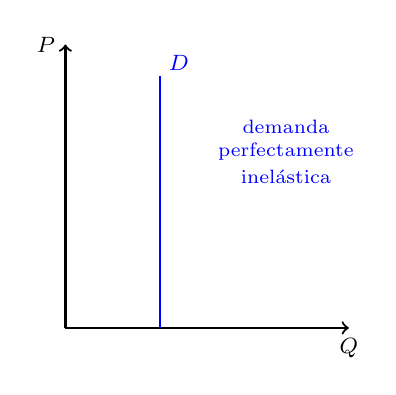
\begin{tikzpicture}[scale=0.8]
      \draw[thick,->] (0,0) -- (4.5,0) node[below] {\footnotesize $Q$};
      \draw[thick,->] (0,0) -- (0,4.5) node[left] {\footnotesize $P$};
      \draw[thick, blue] (1.5,0) -- (1.5,4); % Demanda vertical
      \node[blue] at (1.8,4.2) {\footnotesize $D$};
      \node[blue] at (3.5,3.2) {\scriptsize demanda};
      \node[blue] at (3.5,2.8) {\scriptsize perfectamente};
      \node[blue] at (3.5,2.4) {\scriptsize inelástica};
  
  \end{tikzpicture}
  \end{minipage}
  \hfill
  % Segundo gráfico: demanda inelastica
  \begin{minipage}{0.48\textwidth}
  \centering
  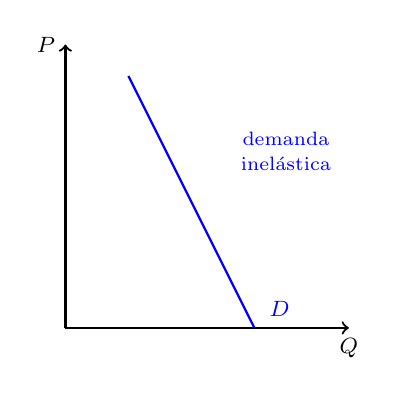
\begin{tikzpicture}[scale=0.8]
      \draw[thick,->] (0,0) -- (4.5,0) node[below] {\footnotesize $Q$};
      \draw[thick,->] (0,0) -- (0,4.5) node[left] {\footnotesize $P$};
      \draw[thick, blue] (1,4) -- (3,0); 
      \node[blue] at (3.4,0.3) {\footnotesize $D$};
      \node[blue] at (3.5,3) {\scriptsize demanda};
      \node[blue] at (3.5,2.6) {\scriptsize inelástica};
  \end{tikzpicture}
  \end{minipage}
  
  \end{figure}
\end{frame}

\begin{frame}{Elasticidad precio de la demanda}
    \begin{itemize}
      \item Si ante un cambio en el precio de un bien, la cantidad demandada cambia en una proporción mayor al cambio proporcional del precio, se dice que la demanda es \textbf{elástica} ($\Delta \% Q >\Delta \% P$)
      \item Esto sucede siempre que la elasticidad sea \textbf{mayor a 1}.
      \item En el caso en el que la elasticidad sea $\infty$, la demanda es \textbf{perfectamente elástica}.
    \end{itemize}
  
  \begin{figure}[h]
  \centering
  % Primer gráfico: demanda  elástica
  \begin{minipage}{0.48\textwidth}
  \centering
  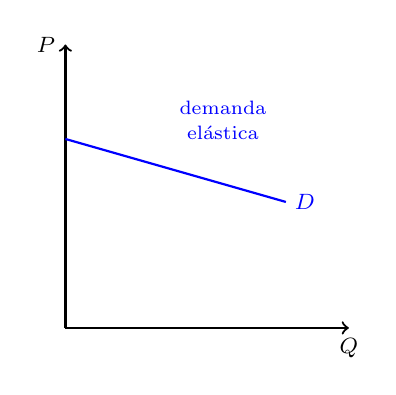
\begin{tikzpicture}[scale=0.8]
      \draw[thick,->] (0,0) -- (4.5,0) node[below] {\footnotesize $Q$};
      \draw[thick,->] (0,0) -- (0,4.5) node[left] {\footnotesize $P$};
      \draw[thick, blue] (0,3) -- (3.5,2); 
      \node[blue] at (3.8,2) {\footnotesize $D$};
      \node[blue] at (2.5,3.5) {\scriptsize demanda};
      \node[blue] at (2.5,3.1) {\scriptsize elástica};
  
  \end{tikzpicture}
  \end{minipage}
  \hfill
  % Segundo gráfico: demanda perfectamente elastica
  \begin{minipage}{0.48\textwidth}
  \centering
  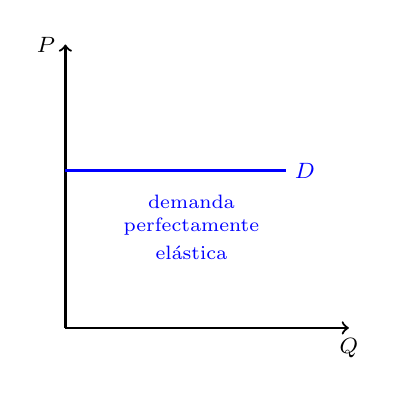
\begin{tikzpicture}[scale=0.8]
      \draw[thick,->] (0,0) -- (4.5,0) node[below] {\footnotesize $Q$};
      \draw[thick,->] (0,0) -- (0,4.5) node[left] {\footnotesize $P$};
      \draw[thick, blue] (0,2.5) -- (3.5,2.5);
      \node[blue] at (3.8,2.5) {\footnotesize $D$};
      \node[blue] at (2,2) {\scriptsize demanda};
      \node[blue] at (2,1.6) {\scriptsize perfectamente};
      \node[blue] at (2,1.2) {\scriptsize elástica};
  
  \end{tikzpicture}
  \end{minipage}
  
  \end{figure}
\end{frame}

\begin{frame}
\frametitle{Elasticidad precio de la demanda}
  \begin{itemize}
    \item Medida de sensibilidad: ¿Cuál es el cambio \% en la cantidad demandada ante un cambio de 1\% en el precio?
    \begin{itemize}
        \item Usamos el modulo para facilitar la interpretación! 
    \end{itemize}
    \item ¿Qué tan elástica?
    \begin{itemize}
      \item Si $\epsilon > 1$ decimos que la demanda es elástica
      \item Si $\epsilon = 1$ decimos que la demanda es unitaria
      \item Si $\epsilon < 1$ decimos que la demanda es inelástica
    \end{itemize}
  \end{itemize}
\end{frame}

\begin{frame}{Determinantes de la elasticidad precio de la demanda}
  \begin{itemize}
    \item \textbf{Disponibilidad de sustitutos cercanos}. Bienes con sustitutos cercanos tienden a tener demandas más elásticas.
    \item \textbf{La necesidad de consumo}. Cuanto más necesario sea el consumo de un bien o servicio, menor capacidad de
    respuesta tendrá el consumidor y más inelástica será la demanda.
    \item \textbf{La temporalidad de ajuste en el consumo}. Mientras más largo
    sea el período temporal que estemos considerando para el ajuste en las cantidades,
    los bienes tienden a tener demandas más elásticas, precisamente
    porque los consumidores pueden ajustar su consumo con el tiempo.
    \item \textbf{Definición de mercado}: mientras más general sea el mercado, se tiende a tener demandas menos elásticas, porque se vuelve más difícil encontrar sustitutos cercanos (mercado de remeras vs. mercado de remeras de River)
  \end{itemize}
\end{frame}

\begin{frame}{Elasticidad Puntual y Pendiente}
    \begin{itemize}
        \item La elasticidad puntual es el valor de la elasticidad precio \textbf{en un punto específico} sobre la curva de demanda.
    \end{itemize}
  \begin{footnotesize}
    \begin{equation*}
      \epsilon = \left|\frac{- \Delta \% Q}{\Delta \% P}\right| = \left|\frac{\frac{- \Delta Q}{Q}}{\frac{\Delta P}{P}}\right| = \left|-\frac{\Delta Q}{\Delta P} \frac{P}{Q}\right|\,\,\,\,\,\,\text{y}\,\,\,\,\,\, \text{pend} = \frac{\Delta P}{\Delta Q}
    \end{equation*}
    
  \end{footnotesize}
  \begin{itemize}
    
    \item La pendiente forma parte del concepto de elasticidad. Una demanda muy empinada es relativamente inelástica, y una bastante plana es elástica.
    \item ¡Ojo! La elasticidad puede cambiar a medida que nos movemos a lo largo de la curva de demanda, aun si la pendiente no lo hace.
  \end{itemize}
    \centering
    \includegraphics[scale=0.35]{../Figures/C16.7.png}
\end{frame}

\begin{frame}{Pendiente constante, elasticidad variable}
    \begin{figure}[h]
    \centering
    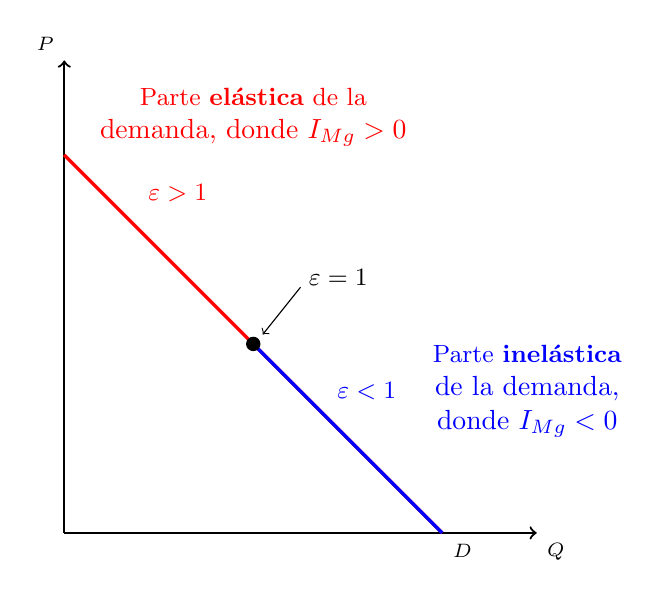
\begin{tikzpicture}[scale=1.2]
    
        % Ejes
        \draw[thick,->] (0,0) -- (5,0) node[below right] {\scriptsize $Q$};
        \draw[thick,->] (0,0) -- (0,5) node[above left] {\scriptsize $P$};
    
        % Curva de demanda
        \draw[very thick, red] (0,4) -- (4,0) node[below right, black] {\scriptsize $D$};
        \draw[very thick, blue] (2,2) -- (4,0);
        
        % Punto de elasticidad unitaria
        \filldraw[black] (2,2) circle (2pt);
        \draw[->] (2.5,2.6) -- (2.1,2.1);
        \node at (2.9,2.7) {\small $\varepsilon = 1$};
    
        % Texto zona elástica
        \node[red] at (1.2,3.6) {\small $\varepsilon > 1$};
        \node[align=center, text=red] at (2,4.4) 
            {\small Parte \textbf{elástica} de la\\demanda, donde $I_{Mg} > 0$};
    
        % Texto zona inelástica
        \node[blue] at (3.2,1.5) {\small $\varepsilon < 1$};
        \node[align=center, text=blue] at (4.9,1.5) 
            {\small Parte \textbf{inelástica} \\de la demanda,\\ donde $I_{Mg} < 0$};
    
    \end{tikzpicture}
    \end{figure}
\end{frame}

\begin{frame}
    \frametitle{Elasticidad constante, pendiente variable}
    
    \begin{figure}[h]
    \centering
    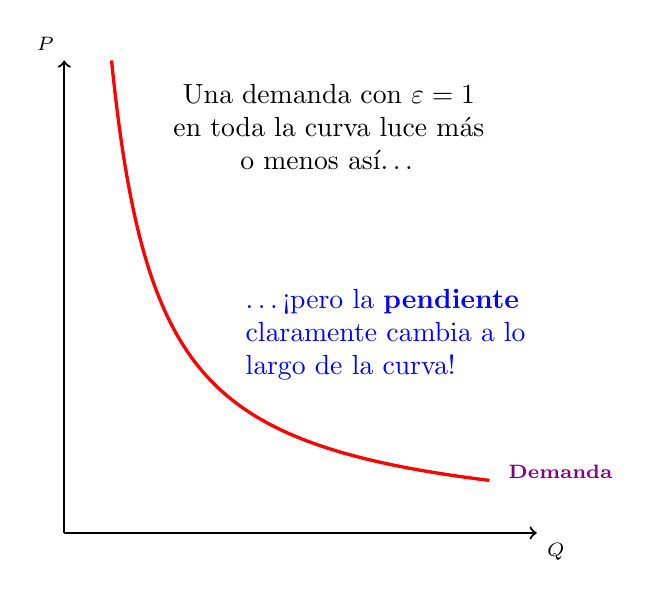
\begin{tikzpicture}[scale=1.2]
    
        % Ejes
        \draw[thick,->] (0,0) -- (5,0) node[below right] {\scriptsize $Q$};
        \draw[thick,->] (0,0) -- (0,5) node[above left] {\scriptsize $P$};
        
        % Curva de demanda (hipérbola equilátera)
        \draw[very thick, red, domain=0.5:4.5, samples=200] 
            plot (\x,{2.5/(\x)});
    
        % Texto arriba explicativo
        \node[align=center] at (2.8,4.3) 
            {Una demanda con $\varepsilon = 1$\\ en toda la curva luce más\\ o menos así…};
    
        % Texto abajo explicativo
        \node[align=left, text=blue] at (3.4,2.1) 
            {\dots ¡pero la \textbf{pendiente}\\ claramente cambia a lo\\ largo de la curva!};
    
        % Etiqueta de la curva
        \node[text=violet, right] at (4.6,0.65) {\scriptsize \textbf{Demanda}};
    
    \end{tikzpicture}
    \end{figure}
\end{frame}
    
% \begin{frame}
%     \frametitle{Elasticidad constante}
%     \includegraphics[scale=0.6]{../Figures/Tema_06.45_elasticidad.png}
% \end{frame}

% \begin{frame}
%   \frametitle{Pendiente constante}
%   \includegraphics[scale=0.6]{../Figures/Tema_06.46_elasticidad2.png}
% \end{frame}

\begin{frame}
\frametitle{Ingreso total y elasticidad}
\begin{itemize}
    \item El impacto de un cambio de precio en los ingresos totales, depende de la elasticidad de la demanda.
    \item Si la demanda es inelástica un incremento en el precio provoca un decremento en la cantidad demandada proporcionalmente más pequeño, por lo cual los ingresos totales se incrementan.
    \item En esa misma demanda, un descenso en el precio provoca un aumento en la cantidad demandada proporcionalmente más pequeño también, por lo cual los ingresos totales disminuyen.
    \item Si la curva de la demanda es elástica, un incremento en el precio provoca una disminución en la cantidad demandada proporcionalmente más grande, por lo que los ingresos totales disminuyen.
    \item En esa misma demanda, un descenso en el precio provoca un aumento en la cantidad demandada proporcionalmente más grande, por lo que los ingresos totales aumentan.
\end{itemize}
\end{frame}

\begin{frame}{Ingreso total y elasticidad}
    \centering
    
    \begin{minipage}{0.48\textwidth}
    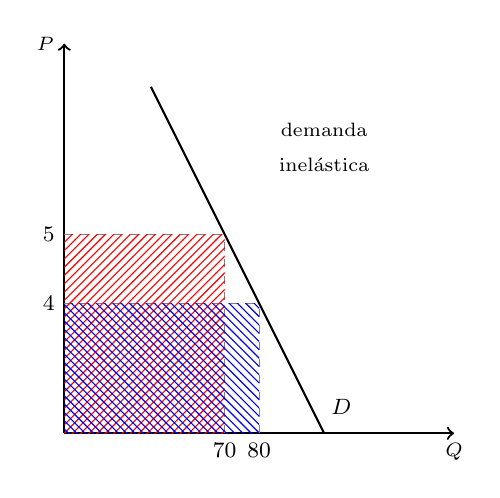
\begin{tikzpicture}[scale=1.1]
        \draw[thick,->] (0,0) -- (4.5,0) node[below] {\scriptsize $Q$};
        \draw[thick,->] (0,0) -- (0,4.5) node[left] {\scriptsize $P$};
        \draw[thick] (1,4) -- (3,0); 
        \node at (3.2,0.3) {\footnotesize $D$};
        \node at (3,3.5) {\scriptsize demanda};
        \node  at (3,3.1) {\scriptsize inelástica};
    
        \draw[dashed, gray] (0,2.3) -- (1.85,2.3);
        \draw[dashed, gray] (1.85,0) -- (1.85,2.3);
        \node[left] at (0,2.3) {\footnotesize $5$};
        \node[below] at (1.85,0) {\footnotesize $70$};
    
        \draw[dashed, gray] (0,1.5) -- (2.25,1.5);
        \draw[dashed, gray] (2.25,0) -- (2.25,1.5);
        \node[left] at (0,1.5) {\footnotesize $4$};
        \node[below] at (2.25,0) {\footnotesize $80$};
    
        \fill[pattern=north east lines,  pattern color=red] (0,0) rectangle (1.85,2.3);
    
        \fill[pattern=north west lines,  pattern color=blue] (0,0) rectangle (2.25,1.5);
    
        %\fill[red!30, opacity=0.5] (0,1.5) rectangle (1.75,2.5);
    
        %\fill[blue!30, opacity=0.5] (1.75,0) rectangle (2.25,1.5);
    \end{tikzpicture}
    \end{minipage}
    \hfill
    \begin{minipage}{0.48\textwidth}
    \centering
    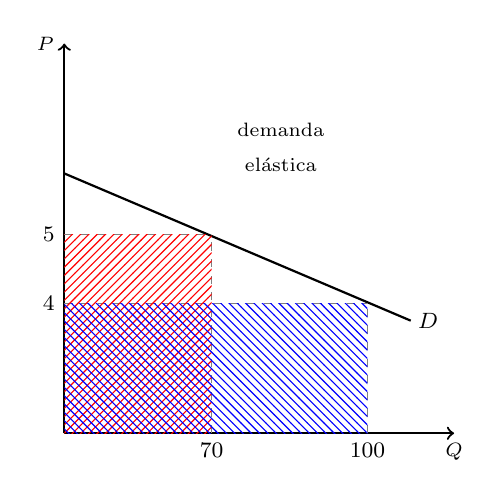
\begin{tikzpicture}[scale=1.1]
        \draw[thick,->] (0,0) -- (4.5,0) node[below] {\scriptsize $Q$};
        \draw[thick,->] (0,0) -- (0,4.5) node[left] {\scriptsize $P$};
        \draw[thick] (0,3) -- (4,1.3); 
        \node[below] at (4.2,1.5) {\footnotesize $D$};
        \node at (2.5,3.5) {\scriptsize demanda};
        \node at (2.5,3.1) {\scriptsize elástica};
    
        \draw[dashed, gray] (0,2.3) -- (1.7,2.3);
        \draw[dashed, gray] (1.7,0) -- (1.7,2.3);
        \node[left] at (0,2.3) {\footnotesize $5$};
        \node[below] at (1.7,0) {\footnotesize $70$};
    
        \draw[dashed, gray] (0,1.5) -- (3.5,1.5);
        \draw[dashed, gray] (3.5,0) -- (3.5,1.5);
        \node[left] at (0,1.5) {\footnotesize $4$};
        \node[below] at (3.5,0) {\footnotesize $100$};
    
        \fill[pattern=north east lines,  pattern color=red] (0,0) rectangle (1.7,2.3);
    
        \fill[pattern=north west lines,  pattern color=blue] (0,0) rectangle (3.5,1.5);
    \end{tikzpicture}
    \end{minipage}
\end{frame}

\begin{frame}{Elasticidad Punto Medio}
  \begin{itemize}
      \item Hay otra forma de calcular la elasticidad, \textbf{la elasticidad punto medio}.
      \item Se utiliza para calcular la elasticidad entre dos puntos
      específicos de la curva de demanda que enfrenta una firma y se define
      de la siguiente manera:
    \end{itemize}
    \begin{equation*}
      \epsilon = \left|\frac{- \Delta \% Q}{\Delta \% P}\right|= \left|\frac{- \Delta Q}{\Delta P} \frac{\bar P}{\bar Q}\right| = \left|\frac{\frac{- \Delta Q}{\frac{(Q_2+Q_1)}{2}}}{\frac{\Delta P}{\frac{(P_2+P_1)}{2}}}\right| = \left|-\frac{\Delta Q}{\Delta P} \frac{\frac{(P_2+P_1)}{2}}{\frac{(Q_2+Q_1)}{2}}\right|
    \end{equation*}
\end{frame}

\begin{frame}
    \frametitle{Elasticidad precio de la oferta}
      \begin{itemize}
        \item Se relaciona con la sensibilidad o grado de reacción que tienen las firmas en la cantidad que ofrecen cuando se produce una variación en el precio
        \begin{equation*}
          \epsilon^{O}_p = \frac{\Delta \% Q}{\Delta \% P} = \frac{\frac{\Delta Q}{Q}}{\frac{\Delta P}{P}} = \frac{\Delta Q}{\Delta P} \frac{P}{Q}
        \end{equation*}
        \vspace{-2mm}
        \begin{itemize}
          \item \textbf{Elástica} ($\epsilon^{O}_p>1$): Un cambio en el precio del bien provoca un cambio
          proporcional mayor en la cantidad ofertada del bien.
          \item \textbf{Inelástica} ($\epsilon^{O}_p<1$): Un cambio en el precio de un bien provoca un cambia proporcionalmente menor en su cantidad ofertada.
          \item \textbf{Unitaria} ($\epsilon^{O}_p=1$): un cambio en el precio se traduce como un cambio en la
          cantidad ofertada en la misma proporción.
          \item \textbf{Perfectamente elástica} implica $\epsilon^{O}_p=\infty$ y \textbf{perfectamente inelástica} implica $\epsilon^{O}_p=0$.
        \end{itemize}
          \item El módulo en este caso no es necesario porque la pendiente es positiva y, por ende, la elasticidad también.
       \end{itemize}
\end{frame}
    
\begin{frame}{Determinantes de la elasticidad precio de la demanda}
      \begin{itemize}
          \item \textbf{Posibilidad de stockearse:} si el bien se puede almacenar, el productor puede ofrecer más cuando sube el precio (mayor elasticidad).    
          \item \textbf{Tiempo de producción:} cuanto más rápido se puede producir un bien, más elástica será la oferta.
          \item \textbf{Procesos productivos:} cuanto más adaptable es la tecnología, más fácil ajustar la producción.
          \item \textbf{Dependencia de insumos:} si el productor depende de insumos importados o escasos, la oferta será más inelástica.
        \end{itemize}
\end{frame}

\begin{frame}{Elasticidad Cruzada}
    \begin{itemize}
        \item Es el cambio porcentual en las cantidades demandadas cuando \textbf{el precio de otro bien} cambia 1\%.
        \begin{equation*}
            \epsilon_{x,y} = \frac{\Delta \% Q_x}{\Delta \% P_y}
        \end{equation*}
            \begin{itemize}
            \item Si la elasticidad cruzada es 0, no hay relación entre ambos bienes.
            \item Si esta elasticidad es mayor a 0, los bienes son sustitutos, es decir, cuando se incrementa el precio de y aumenta la cantidad demandada de x; 
            \item Si es menor a 0, los bienes son complementarios, es decir, si aumenta el precio de y baja la cantidad demandada de x.
            \end{itemize}
        \item En este caso, es necesario no usar módulo porque es justamente el signo lo que nos ayuda a interpretar qué tipo de bienes son.
    \end{itemize}
\end{frame}

\begin{frame}{Elasticidad Ingreso}
  \begin{itemize}
    \item Es el cambio porcentual en las cantidades demandadas cuando el \textbf{ingreso} cambia 1\%.
    \begin{equation*}
      \epsilon_I = \frac{\Delta \% Q}{\Delta \% I}
    \end{equation*}    
    \begin{itemize}
        \item Si la elasticidad ingreso es mayor a 0, significa que ingreso y cantidades se mueven en conjunto, por lo que se trata de bienes normales.
        \item Si la elasticidad ingreso es menor a cero, ante un cambio en el ingreso la cantidad demandada del bien se mueve en la dirección opuesta. En este caso estamos en presencia de un bien inferior.
        \item Si la elasticidad ingreso es mayor a 1 decimos que estamos ante un bien de lujo.
    \end{itemize}
    \item  En este caso, al igual que con la elasticidad cruzada, es necesario no usar módulo porque es justamente el signo lo que nos ayuda a interpretar qué tipo de bienes son.
\end{itemize}
\end{frame}


\end{document}